\documentclass[14pt]{beamer}
\usetheme{Montpellier}
\usecolortheme{beaver}

\usepackage{amsmath, amssymb, ../../vimacros, hyperref, enumerate}
\usepackage[round]{natbib}

\hypersetup{breaklinks=true, colorlinks=true, linkcolor=blue, citecolor=blue, urlcolor=blue}

\usepackage{tikz}
\usetikzlibrary{bayesnet}

\beamertemplatenavigationsymbolsempty

\title{Variational Inference: Introduction}
\date{}
\author[Schulz and Aziz]{Philip Schulz and Wilker Aziz \\
\url{https://github.com/philschulz/VITutorial}}

\setbeamertemplate{footline}[frame number]

\begin{document}

\frame{\titlepage}

\frame{\tableofcontents}

%\section{Generative Models}
%\frame{\tableofcontents[currentsection]}

\begin{frame}{Problems}


%\begin{small}

Supervised problems: \alert{``learn a mapping from this to that''}
\begin{itemize}
	\item \textcolor{gray}{e.g. machine translation, syntactic parsing, semantic role labelling, image captioning, ...}
\end{itemize}

~

Unsupervised problems: \alert{``learn a distribution that generates the data with high probability''}
\begin{itemize}
	\item \textcolor{gray}{sentences in natural language, images, videos, ...}
\end{itemize}


%\end{small}

\end{frame}



\begin{frame}{Maximum likelihood estimation}

\small

We have data $x^{(1)}, \ldots, x^{(N)}$ e.g.  \\
\begin{itemize}
	\item sentences, images, ...
\end{itemize}
generated by some {\bf unknown} procedure

\pause

which we assume can be captured by a probabilistic model
\begin{itemize}
	\item with {\bf known} probability (mass/density) function e.g.
	\begin{align*}
    X \sim \Cat(\alert{\pi_1}, \alert{\ldots}, \alert{\pi_K}) & & \text{or} & & X \sim \mathcal N(\alert\mu, \alert\sigma^2)
    \end{align*}    
\end{itemize}
and proceed to \alert{estimate parameters} that assign maximum likelihood to observations

\end{frame}



\begin{frame}{Where does deep learning kick in?}

Let $\phi$ be all side information available\\
~ e.g. deterministic \emph{inputs/features}

~

Have neural networks predict parameters of our probabilistic model
	\begin{align*}
    X|\phi \sim \Cat(\pi_{\alert w}(\phi)) & & \text{or} & & X|\phi \sim \mathcal N(\mu_{\alert w}(\phi), \sigma_{\alert w}(\phi)^2)
    \end{align*}
~ and proceed to \alert{estimate parameters} $w$ of the NNs %via MLE % that assign maximum likelihood to observations

 





\end{frame}



\begin{frame}{Multiple problems, same language}



\begin{small}

\begin{columns}
\begin{column}{0.3\textwidth}
\scalebox{0.8}{
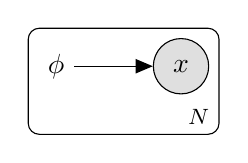
\begin{tikzpicture}
\node[obs] (x) {$ x $};
\node[left=of x] (phi) {$ \phi $};

\edge{phi}{x};

\plate {data} {(x)(phi)} {$ N $};
\end{tikzpicture}
}
\end{column}
\begin{column}{0.6\textwidth}
\alert{(Conditional) Density estimation}
\end{column}

\end{columns}

\begin{tabular}{p{2cm} p{4cm} p{4cm}}
 & $\phi$ & $x$ \\
Parsing &   \textcolor{gray}{a sentence} & \textcolor{black}{its syntactic/semantic parse tree/graph} \\
&&\\
Translation &  \textcolor{gray}{a sentence} & \textcolor{black}{its translation} \\
&&\\
Captioning &  \textcolor{gray}{an image} & \textcolor{black}{caption in English} \\
&&\\
Entailment  & \textcolor{gray}{a text and hypothesis} & \textcolor{black}{entailment relation}
\end{tabular}
\end{small}

\end{frame}


\begin{frame}{Task-driven feature extraction}

Often our side information $\phi$ is itself some high dimensional data
\begin{itemize}
	\item $\phi$ is a sentence and $x$ a tree
	\item $\phi$ is the source sentence and $x$ is the target
	\item $\phi$ is an image and $x$ is a caption
\end{itemize}
and part of the job of the NNs that parametrise our models is to also \alert{deterministically} encode that input in a low-dimensional space

%~
%\begin{itemize}
%	\item NNs parameterise probability functions
%	\item NNs predict parameters of a probabilistic model
%\end{itemize}

\end{frame}


\begin{frame}{NN as efficient parametrisation}

From the statistical point of view NNs do not generate data\\
\begin{itemize}
	\item \alert{they parametrise distributions} that \\
	\emph{by assumption} govern data
\end{itemize}


Compact and efficient way to \alert{map from complex side information to parameter space}

\vspace{10pt}


Prediction is done by a decision rule outside the statistical model
\begin{itemize}
	\item e.g. beam search
\end{itemize}

\end{frame}


\begin{frame}{MLE via gradient-based optimisation}

The probability of an observation $X=x$ is given by some \alert{differentiable} probability function
\begin{itemize}
	\item the parameters of which are predicted by $f_w$\\
	\emph{(also differentiable)}
\end{itemize}

Example: $K$ classes
\begin{small}
\begin{equation*}
\Cat(X=x|f_w(\phi)) = \prod_{i=1}^K f_w(\phi)^{[x=i]} 
\end{equation*}
%\begin{equation*}
%\mathcal N(X=x|\mu_w(\phi), \sigma_w(\phi)^2) = \frac{1}{\sqrt{2\pi\sigma_w(\phi)^2}}\exp\left(-\frac{(x - \mu_w(\phi))^2}{2\sigma_w(\phi)^2}\right)
%\end{equation*}
\end{small}

Given a dataset of i.i.d. observations, SGD gives us a local optimum of the log-likelihood %surface %via stochastic optimisation


\end{frame}



\begin{frame}{DL in NLP recipe}


%Vast majority of papers published at ACL

%\begin{small}
%\begin{figure}
%\scalebox{0.8}{
%\begin{tikzpicture}
%\node[obs] (x) {$ x $};
%\node[left=of x] (phi) {$ \phi $};
%\factor[left=of x] {f} {below:$f_w$} {phi} {x} ; 
%%\edge{phi}{x} ;
%\plate {data} {(x)(phi)} {$ N $};
%\end{tikzpicture}
%}
%\end{figure}
%\end{small}
	Maximum likelihood estimation
	\begin{itemize}
		\item  tells you which \alert{loss} to optimise \\
		(i.e. negative log-likelihood)
	\end{itemize}
	
	Automatic differentiation (\emph{backprop})
	\begin{itemize}
		\item ``give me a tractable forward pass and I will give you \alert{gradients}''
	\end{itemize}
	
	Stochastic optimisation powered by backprop
	\begin{itemize}
		\item general purpose gradient-based optimisers
	\end{itemize}

\end{frame}


\begin{frame}{Tractability is central}

Likelihood gives you a differentiable objective to optimise for
\begin{itemize}
	\item but we need to stick with \alert{tractable} likelihood functions
\end{itemize}



%, any intractable likelihood will leave us in bad territory because
%\begin{itemize}
%	\item stochastic optimisation requires gradient estimates
%	\item which must be unbiased (forget greedy techniques)
%	\item and some estimation techniques are not differentiable (forget MC sampling)
%\end{itemize}

\end{frame}

\begin{frame}{When do have intractable likelihood?}

Latent variables: assessing the likelihood requires marginalisation
\begin{itemize}
	\item too many forward passes
	\begin{small}
	\begin{equation*}
	P_X(x|\phi) = \sum_{c=1}^K \Cat(c|\pi_1, \ldots, \pi_K) \underbrace{\mathcal N(x|\mu_w(c), \sigma_w(c)^2)}_{\text{forward pass}}
	\end{equation*}
	\end{small}
	\item even infinitely many
	\begin{small}
	\begin{equation*}
	P_X(x|\phi) = \int \mathcal N(z|0, I) \underbrace{\Cat(x|\pi_w(z))}_{\text{forward pass}} \mathrm{d}z
	\end{equation*}
	\end{small}
\end{itemize}

\end{frame}


\begin{frame}{But I know approximations!}

Beam-search % for discrete latent variables
\begin{itemize}
	\item stochastic optimisation requires \alert{unbiased gradient estimates}
\end{itemize}

~

Monte Carlo sampling
\begin{itemize}
	\item \alert{breaks differentiability} (bye bye backprop)
\end{itemize}

\end{frame}


\begin{frame}{What do we do then?}

Vast majority of papers published at ACL

\begin{small}
\begin{figure}
\scalebox{0.8}{
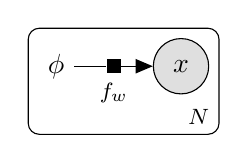
\begin{tikzpicture}
\node[obs] (x) {$ x $};
\node[left=of x] (phi) {$ \phi $};
\factor[left=of x] {f} {below:$f_w$} {phi} {x} ; 
%\edge{phi}{x} ;
\plate {data} {(x)(phi)} {$ N $};
\end{tikzpicture}
}
\end{figure}
\end{small}
\begin{itemize}
	\item encode more and more inductive bias through the design of the architecture
	\begin{itemize}
		\item and what if we want to learn clusters?
		\item or segmentation?
		\item or sparse embeddings?
		\item or sparse models?
		\item or latent factors?
	\end{itemize}
\end{itemize}

\end{frame}

\begin{frame}{Deep Generative Models}

Probabilistic models parametrised by neural networks
\begin{itemize}
	\item better modelling assumptions\\
	one of the reasons why there's so much interest	
	\item but requires efficient inference\\
	\alert{which is the reason why we are here today}
\end{itemize}

\end{frame}


%\nocite{BleiEtAl:2016}
%\nocite{NealHinton:1998}
%\nocite{GhahramaniJordan:1996}
%\nocite{BleiEtAl:2003}

\begin{frame}[allowframebreaks]{Literature}
\bibliographystyle{plainnat}
\small
\bibliography{../../VI}
\end{frame}

\end{document}
